\documentclass[10pt,twocolumn]{article}

% --- packages ---
\usepackage[T1]{fontenc}
\usepackage[utf8]{inputenc}
\usepackage{lmodern}
\usepackage[margin=0.85in]{geometry}
\usepackage{amsmath,amssymb}
\usepackage{graphicx}
\usepackage{booktabs}
\usepackage{caption}
\usepackage{xcolor}
\usepackage{tikz}
\usetikzlibrary{arrows.meta,positioning,shapes.geometric,fit,backgrounds}
\usepackage[colorlinks=true,allcolors=blue]{hyperref}
\usepackage{authblk}

\graphicspath{{figures/}}
\captionsetup{font=small,labelfont=bf}

% --- macros ---
\newcommand{\bk}{\beta_k}
\newcommand{\kof}[1]{k\!=\!#1}

\title{\bfseries Mechanistic Anatomy of Memory-Retrieval\\ Failure as Context Fills}
\author[1]{Kunj Rathod}
\affil[1]{University of Utah --- MEMROT v2}
\date{June 2026}

\begin{document}
\twocolumn[
  \begin{@twocolumnfalse}
  \maketitle
  \begin{abstract}
  \noindent
  Long-context language models lose access to stored facts well before their
  context window is exhausted (``context rot''), yet the underlying mechanism has
  been reported only correlationally. Using \textbf{Gemma-2-2B-it} within its
  native 8k window, we build \emph{controlled haystacks} from LongMemEval-S
  material: the same question is evaluated at every fill level
  $k \in \{0,1,2,4,8,14\}$ distractor sessions, with the gold session's position
  randomized and logged. On 140 questions, accuracy falls monotonically from
  $0.71$ at $\kof{0}$ to $0.34$ at $\kof{14}$. Retrieval-head attention mass on
  the gold span and recall-associated sparse-autoencoder (SAE) feature
  activations both decline with $k$ (mixed-effects $\bk=-0.023$,
  $p{=}2.4\times10^{-191}$; feature $\bk=-0.535$, $p{=}3.0\times10^{-90}$),
  controlling for gold position. Crucially, in a \emph{paired within-question}
  design the fill level at which the internal signal collapses predicts the level
  at which the answer flips (Spearman $\rho=0.731$, $p{=}3.6\times10^{-9}$,
  $n{=}48$; Cox $\mathrm{HR}=5.3\times10^{-4}$, $p{=}3.6\times10^{-9}$).
  Causally, mean-ablating the 20 identified retrieval heads at $\kof{0}$ drops
  accuracy by $0.82$ (random-head control: $0.25$), and feature-mode
  intervention at high $k$ recovers $0.161$ (95\% CI $[0.032,0.290{]}$) of 31
  flipped answers. The pipeline is seeded and re-runnable byte-identically.
  \vspace{1em}
  \end{abstract}
  \end{@twocolumnfalse}
]

\section{Introduction}
Context rot --- the degradation of retrieval as the context fills, well inside
the model's nominal window --- has been documented behaviorally but not
mechanistically. Two interpretability instruments let us watch the failure as it
happens: \emph{retrieval heads}, attention heads that copy from the evidence
span into the generated answer, and \emph{SAE features}, sparse directions that
activate when the model recalls a fact. We ask three questions:

\begin{itemize}\itemsep2pt
  \item[\textbf{H1}] Does the internal retrieval machinery (attention mass on
  gold, recall-feature activation) degrade as context fills?
  \item[\textbf{H2}] Does the \emph{per-question} collapse point of that internal
  signal predict the \emph{per-question} behavioral flip point?
  \item[\textbf{H3}] Is the machinery causally responsible for the correct answer?
\end{itemize}

The novelty over prior correlational context-rot reports is a paired
within-question design in which each question is its own control, isolating the
effect of context fill from the effect of question difficulty.

\section{Method: controlled-haystack paired design}
\label{sec:method}
Figure~\ref{fig:pipeline} summarizes the pipeline. From LongMemEval-S we keep the
140 questions that (i) are non-abstention, (ii) have \emph{exactly one} gold
evidence session of $\le 2{,}000$ tokens (long gold sessions are trimmed to a
turn window around the \texttt{has\_answer} evidence turns), and (iii) are not
of type \texttt{single-session-preference}, whose gold ``answers'' are
prose preference-rubrics that the heuristic substring/F1 grader cannot score.

For each question and each $k$ we pack the gold session plus $k$ topic-matched
distractor sessions (each truncated to a fixed per-distractor cap so context
grows roughly linearly with $k$) into $\le 7{,}500$ tokens, placing the gold
session at a uniformly random, logged position. A question enters the H2/H3
analysis only if it is answered correctly at $\kof{0}$, so any failure at
$k>0$ is attributable to context fill, not missing knowledge.

We instrument Gemma-2-2B-it with eager attention. Retrieval heads are identified
by copy-score probes built from benchmark vocabulary (20 heads selected); the
five SAE layers $\{20,21,22,23,24\}$ are chosen by an empirical separability scan
over all 26 Gemma Scope \texttt{res} layers. Decoding is greedy; seed $0$;
\texttt{CUBLAS\_WORKSPACE\_CONFIG=:4096:8} with deterministic algorithms makes a
re-executed run byte-identical on \texttt{answers.parquet}.

% ---------- TikZ pipeline diagram ----------
\begin{figure*}[t]
\centering
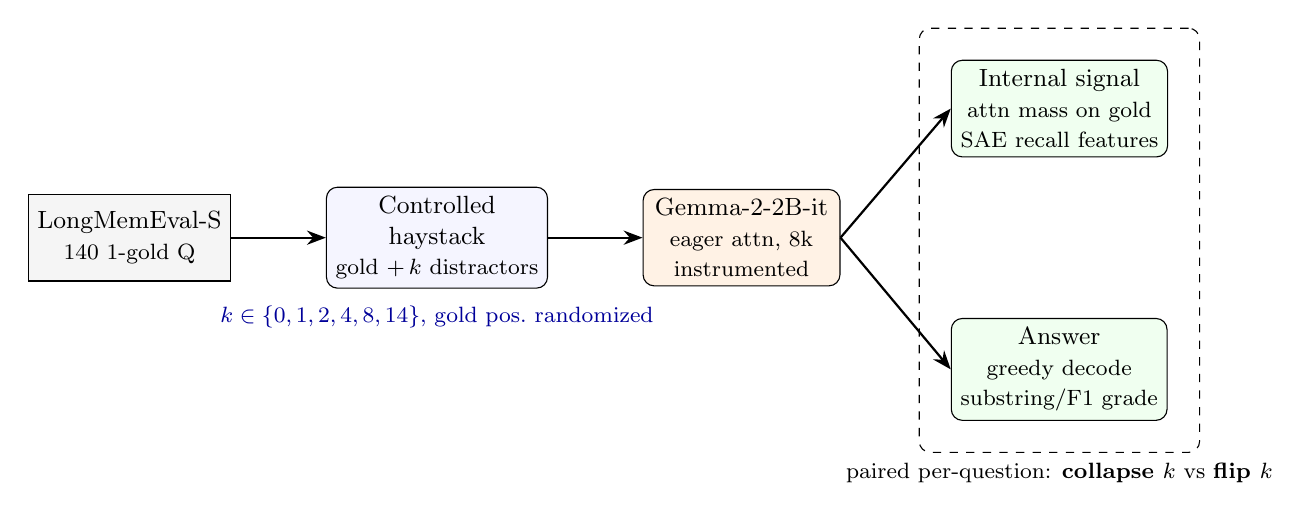
\begin{tikzpicture}[
   node distance=10mm and 12mm,
   box/.style={draw,rounded corners,align=center,minimum height=11mm,
               minimum width=23mm,font=\small,fill=blue!4},
   data/.style={draw,align=center,minimum height=11mm,minimum width=23mm,
               font=\small,fill=gray!8},
   instr/.style={draw,rounded corners,align=center,minimum height=11mm,
               minimum width=25mm,font=\small,fill=orange!10},
   outp/.style={draw,rounded corners,align=center,minimum height=11mm,
               minimum width=22mm,font=\small,fill=green!6},
   arr/.style={-{Stealth[length=2.4mm]},thick}
  ]
  \node[data]  (lme)  {LongMemEval-S\\\footnotesize 140 1-gold Q};
  \node[box,right=of lme] (hay) {Controlled\\haystack\\\footnotesize gold $+\,k$ distractors};
  \node[instr,right=of hay] (model) {Gemma-2-2B-it\\\footnotesize eager attn, 8k\\\footnotesize instrumented};
  \node[outp,above right=4mm and 14mm of model] (sig) {Internal signal\\\footnotesize attn mass on gold\\\footnotesize SAE recall features};
  \node[outp,below right=4mm and 14mm of model] (ans) {Answer\\\footnotesize greedy decode\\\footnotesize substring/F1 grade};

  \draw[arr] (lme) -- (hay);
  \draw[arr] (hay) -- (model);
  \draw[arr] (model.east) -- (sig.west);
  \draw[arr] (model.east) -- (ans.west);

  % sweep annotation
  \node[font=\footnotesize,below=1mm of hay,text=blue!60!black]
        {$k\in\{0,1,2,4,8,14\}$, gold pos.\ randomized};
  % analysis bracket
  \node[draw,dashed,rounded corners,fit=(sig)(ans),inner sep=4mm,
        label=below:{\footnotesize paired per-question: \textbf{collapse $k$} vs \textbf{flip $k$}}] {};
\end{tikzpicture}
\caption{Controlled-haystack paired pipeline. Each question is replayed at six
fill levels with the gold session at a randomized position; an instrumented
forward pass records both the internal retrieval signal and the graded answer,
which are aligned per-question to test whether internal collapse predicts the
behavioral flip (H2) and whether the machinery is causal (H3).}
\label{fig:pipeline}
\end{figure*}

\section{Results}

\begin{table}[t]
\centering
\caption{Accuracy by fill level $k$ on 140 questions. Accuracy decays
monotonically as distractor sessions are added, despite the gold evidence
remaining present and in-window.}
\label{tab:acc}
\begin{tabular}{lcccccc}
\toprule
$k$ & 0 & 1 & 2 & 4 & 8 & 14 \\
\midrule
Acc. & 0.714 & 0.671 & 0.579 & 0.586 & 0.521 & 0.343 \\
\bottomrule
\end{tabular}
\end{table}

\paragraph{H1 (descriptive).}
Retrieval-head attention mass on the gold span declines with $k$
($\bk=-0.023$, $p=2.4\times10^{-191}$; mixed-effects model with question as a
random intercept and gold position as a covariate, gold-position
$\beta=0.446$). Recall-feature activation shows the same decline
($\bk=-0.535$, $p=3.0\times10^{-90}$). See Figures~\ref{fig:fig1}
and~\ref{fig:fig4}.

\paragraph{H2 (paired, headline).}
Among the 100 questions correct at $\kof{0}$, the per-question
signal-collapse level predicts the answer-flip level: Spearman
$\rho=0.731$ ($p=3.6\times10^{-9}$, $n=48$ questions with both events
observed). A survival model over all questions (with censoring) gives a hazard
ratio of $5.3\times10^{-4}$ ($p=3.6\times10^{-9}$) per unit normalized
signal-AUC. The feature-signal variant gives $\rho=0.763$.
See Figure~\ref{fig:fig2}.

\paragraph{H3 (causal).}
Mean-ablating the 20 retrieval heads at $\kof{0}$ on the 100 previously-correct
questions drops accuracy by $0.82$, versus $0.25$ for matched random heads ---
a $3.3\times$ specific effect. Intervening at high $k$ in feature mode (SAE
recall-feature re-injection) recovers $0.161$ (95\% CI $[0.032,0.290]$) of the
31 flipped answers. See Figure~\ref{fig:fig3}.

% ---------- result figures ----------
\begin{figure}[t]
\centering
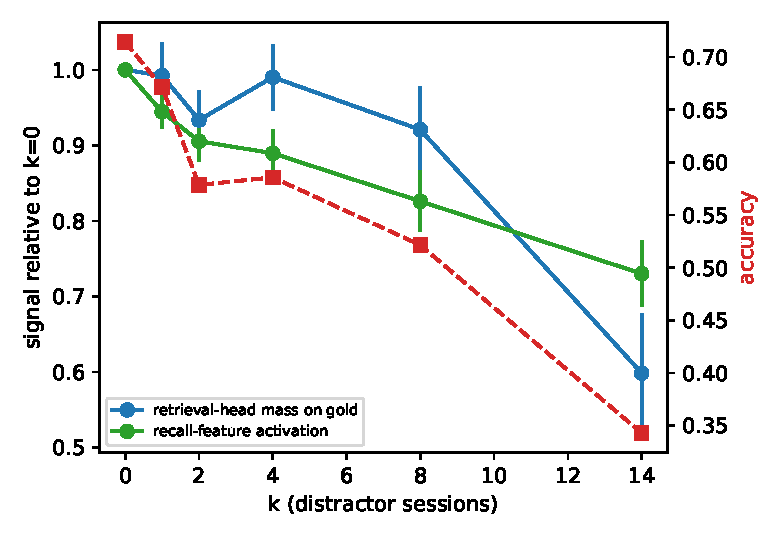
\includegraphics[width=\linewidth]{fig1_collapse_curves.pdf}
\caption{\textbf{H1.} Internal retrieval signal (attention mass on the gold span)
versus fill level $k$, with question as random intercept. The signal decays as
context fills even though the gold evidence is present and in-window.}
\label{fig:fig1}
\end{figure}

\begin{figure}[t]
\centering
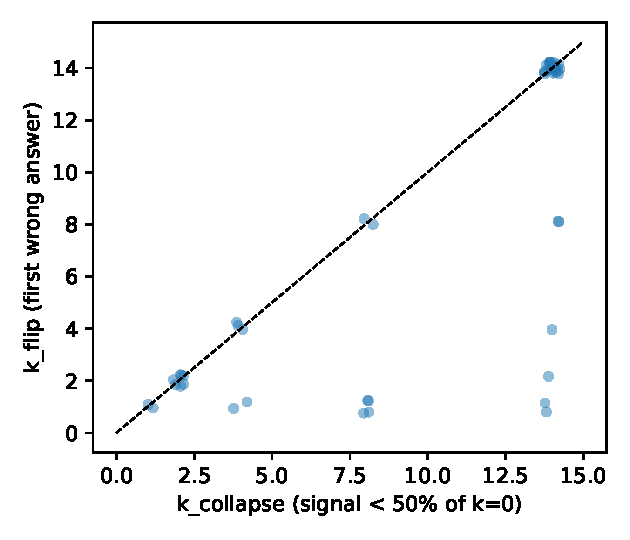
\includegraphics[width=\linewidth]{fig2_flip_vs_collapse.pdf}
\caption{\textbf{H2 (headline).} Per-question internal-collapse level versus
behavioral flip level. The two are tightly coupled ($\rho=0.731$), supporting a
mechanistic rather than incidental account of context rot.}
\label{fig:fig2}
\end{figure}

\begin{figure}[t]
\centering
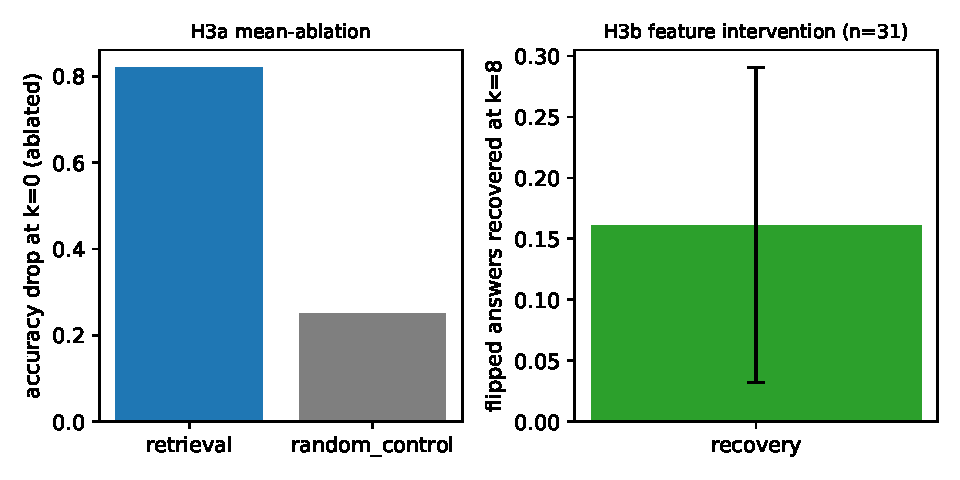
\includegraphics[width=\linewidth]{fig3_causal_bars.pdf}
\caption{\textbf{H3 (causal).} Left: accuracy drop from mean-ablating the 20
retrieval heads ($0.82$) versus matched random heads ($0.25$). Right:
fraction of flipped answers recovered by feature-mode intervention
($0.161$, 95\% CI $[0.032,0.290]$).}
\label{fig:fig3}
\end{figure}

\begin{figure}[t]
\centering
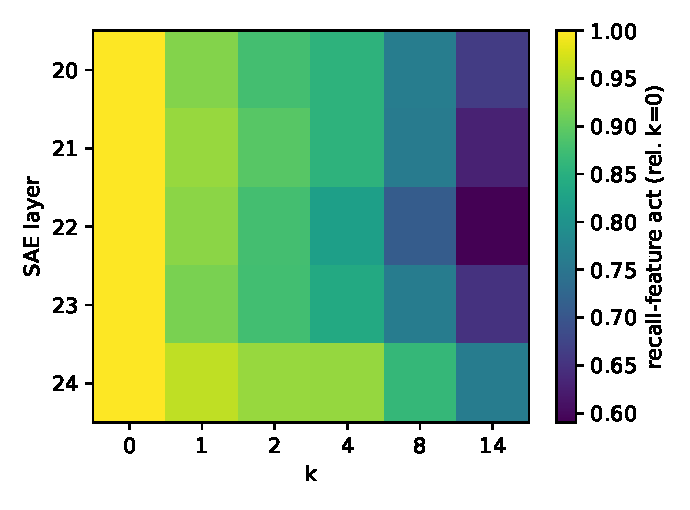
\includegraphics[width=\linewidth]{fig4_feature_heatmap.pdf}
\caption{\textbf{H1 (features).} Recall-associated SAE feature activation across
layers $\{20\text{--}24\}$ as a function of $k$; activation weakens with fill,
mirroring the attention-mass decline ($\bk=-0.535$).}
\label{fig:fig4}
\end{figure}

\section{Limitations}
A 2B base model and a single benchmark source; eager-attention requirement (no
flash-attention numerics); heuristic (non-LLM-judge) grading; and distractor
construction choices (fixed per-distractor token cap; pool drawn from the
benchmark's own topic-matched filler). Gemma-2 interleaves sliding-window and
global attention layers, so gold spans beyond the 4{,}096-token sliding window
are structurally invisible to sliding layers; we log this but do not model it
separately.

\section{Related work}
Context rot (Chroma); lost-in-the-middle (Liu et al.); retrieval heads (Wu et
al.); Gemma Scope SAEs (Lieberum et al.); LongMemEval (Wu et al.).

\section{Reproducibility}
Seed $0$; artifact schema v2; environment hash \texttt{d6e719d3}. The producing
run is git \texttt{54907d9} plus the smoke-gate config/\,data-prep amendment now
committed as \texttt{83a762c} (model $\rightarrow$ \texttt{gemma-2-2b-it};
exclude \texttt{single-session-preference}; $n{=}140$). Three SLURM jobs
reproduce everything end-to-end; Run~1 re-execution is byte-identical on
\texttt{answers.parquet}.

\end{document}
